\chapter{牛顿定律 动量定理}

\section*{A 组}
\vspace{0.3cm}
\textbf{2-1} 如图所示, 一轻绳跨过光滑的定滑轮, 绳的两端等高处分别有一个胖猴和瘦猴, 两猴身高相同. 胖猴使劲沿着绳向上爬, 瘦猴懒洋洋地挂在绳上, 试问吊在滑轮下边的香蕉将归谁所有?


\begin{center}
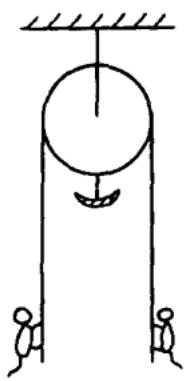
\includegraphics[width=0.1\textwidth]{figures/图2_1.jpg}
\end{center}

\vfill

\textbf{2-2} 天花板下悬挂轻质光滑小圆环 $P, P$ 可绕着过悬挂点的竖直轴无摩擦地旋转，长为 $L$ 的轻绳穿过 $P$ ，两端分别连接质量 $m_{1}$ 和 $m_{2}$ 的小球. 设两球同时作图2-2所示的圆锥摆运动，且在任意时刻两球和绳均在同一个竖直平面内，试求两小球各自到 $P$ 点的距离 $l_{1}$ 和 $l_{2}$ .


\begin{center}
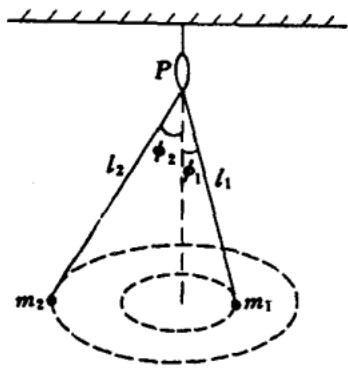
\includegraphics[width=0.2\textwidth]{figures/图2_2.jpg}
\end{center}

\vfill

\newpage

\textbf{2-3} 质量 $m$, 长 $l$ 的匀质细杆 OA, 在光滑的水平面上绕其固定端 $O$ 旋转, 旋转角速度为 $\omega$ 常量. 以 $O$ 端为原点, 在杆上建立沿 OA 方向的 $x$ 轴, 试求细杆中张力 $T$ 随 $x$ 的分布函数.

\vfill

\textbf{2-4} 估算月球中心到地球中心的距离 $r$.


\vfill

\newpage

\textbf{2-5} $A$, $B$ 两本书各 300 张, 每张质量 3 $g$, 纸间摩擦因数同为 $\mu=0.3$ . 将 $A$, $B$ 两书逐张交叠放在光滑水平桌面上, 试问为将两书水平拉开至少要用多大的力?


\vfill

\textbf{2-6} 如图所示,传送带水平段长度为 $l$,传动速度为 $v_{0}$ ,小物块无水平初速地放在传送带的左端,经时间 $t$ 到达右端.已知小物块与传送带之间的摩擦因数处处相同,试求小物块到达右端时的速度 $v$ 及摩擦因数 $\mu$ .


\begin{center}
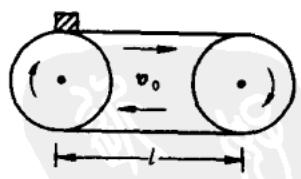
\includegraphics[width=0.2\textwidth]{figures/图2_5.jpg}
\end{center}

\vfill

\newpage

\textbf{2-7} 底圆半顶角为 $\theta$ 的圆锥形筒水平倒置，绕其竖直中央轴以恒定的角速度 $\omega$ 旋转，在筒内侧面距筒顶 $l$ 处放一小物块，如图所示.设物块与筒间摩擦因数为 $\mu$ ，试问 $l$ 取何值时，小物块能相对筒静止？

\begin{center}
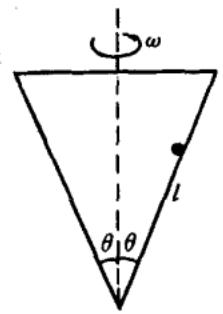
\includegraphics[width=0.15\textwidth]{figures/图2_6.jpg}
\end{center}

\vfill

\textbf{2-8} 将小物块放在水平转盘距中心 $r_{1}=0.10\ m$ 处，转盘以 $\beta=20\ rad/s^{2}$ 的角加速度绕着过中心的竖直轴旋转，当角速度达到 $\omega=7.0\ rad/s$ 时，小物块开始滑动。如果小物块开始时放在距盘心 $r_{2}=0.15\ m$ 处，摩擦因数不变，盘的旋转情况同前，问达到多大角速度 $\omega_{2}$ 时，小物块开始滑动？


\vfill

\newpage

\textbf{2-9} 高台跳水运动员入水后, 当向下的速度降到约 $2 \mathrm{~m} / \mathrm{s}$ 时翻身, 并以双脚蹬池底向上浮出水面为宜. 运动员在水中所受阻力可近似表述为 $\frac{1}{2} C \rho S v^{2}$ , 其中 $C = 0.5$ 是阻力系数, $\rho$ 是人体密度, $S$ 是人体垂直于运动方向的截面积, $v$ 是运动速率, 试为女子 $10 \mathrm{~m}$ 高台跳水设计游泳池的深度.


\vfill

\textbf{2-10} 如图所示, 光滑的水平面上放一个大三角形木块, 在木块的光滑斜面上放一个小长方木块. 将两者从静止自由释放, 试利用平移惯性力建立小长方木块相对大三角形木块的动力学方程, 以协助判定小长方木块到达地面前是否会离开大木块.

\begin{center}
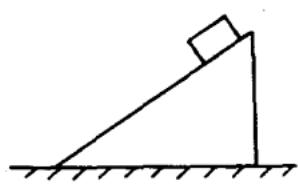
\includegraphics[width=0.2\textwidth]{figures/图2_8.jpg}
\end{center}

\vfill

\newpage

\textbf{2-11} 车厢内的滑轮装置如图所示, 滑轮固定不转动, 只是为轻绳提供光滑的接触. 物块 $A$ 与水平桌面间摩擦因数 $\mu=0.25$ , $A$ 的质量 $m_{A}=20\ kg$ , 物块 $B$ 的质量 $m_{B}=30\ kg$ . 今使车厢沿图示水平朝左方向匀加速运动, 加速度 $a_{0}=2\ m/s^{2}$ , 稳定后绳将倾斜不晃, 试求绳中张力 $T$.

\begin{center}
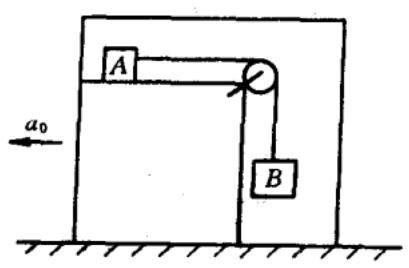
\includegraphics[width=0.25\textwidth]{figures/图2_10.jpg}
\end{center}

\vfill

\textbf{2-12} 游乐场中的转笼是一个半径 3 $m$ 的直立圆筒, 可绕中央竖直轴旋转, 游客可背靠筒壁站立在水平踏板上, 筒壁上有粗糙的网纹以增大游客与筒壁之间的摩擦因数 $\mu$ . 当转速达到每分钟 30 转时, 游客脚下踏板脱落, 从转笼参考系考虑, 为使游客不会掉下落地, 试问 $\mu$ 至少为多大?


\vfill

\newpage

\textbf{2-13} 不计空气阻力, 近似计算小球从赤道上空 100 $m$ 高处自由下落时, 因受科里奥利力影响产生的落地偏东值. (数学处理时,可利用复合函数微商链锁法则： $\frac{\mathrm{d}y}{\mathrm{d}x} = \frac{\mathrm{d}y}{\mathrm{d}u} \frac{\mathrm{d}u}{\mathrm{d}x}$)


\vfill

\textbf{2-14} 以角速度 $\omega$ 绕着过中心竖直轴匀速旋转的水平大圆盘上有一弦心距为 $d$ 的足够长直弦槽，槽内有一个质量 $m$ 的小物块从槽的中央 $O$ 处以初始相对速率 $v_{0}$ 沿槽运动。已知小物块与槽的侧壁光滑接触，与槽底间的摩擦因数为 $\mu$ 。试问 $\mu$ 为何值，小物块最终能停住？再设所给 $\mu$ 值能使小物块停住，试导出小物块滑动时槽的侧壁所受正压力大小 $N$ 与物块经过的路程 $x$ 之间的关系，并计算小物块通过的总路程 $s$ 。

\vfill

\newpage

\textbf{2-15} 半长轴为 $a$、半短轴为 $b$ 的椭圆，长轴端点处的曲率半径 $\rho=b^{2}/a$ .质量 $m$ 的人造卫星绕地球作椭圆运动, 近地点离地面的高度为 2R, 远地点离地面的高度为 3R, 其中 $R$ 是地球半径. 已知地球表面处重力加速度为 $g$, 试求人造卫星从远地点到近地点运行过程中, 地球万有引力给它的总冲量大小 $I$.

\vfill

\textbf{2-16} 光滑水平地面上有一个倾角 $\phi$ 、高 $H$ 、质量 $M$ 的劈形木块, 它的顶部有一质量 $m$ 的小物块, 两者间有摩擦. 开始时系统静止, 如图所示, 而后小物块能够沿斜面下滑到底部, 试求过程中劈形木块在地面上通过的路程 $s$.

\begin{center}
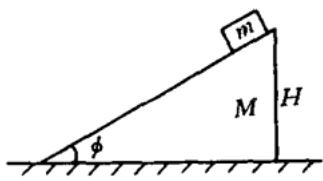
\includegraphics[width=0.2\textwidth]{figures/图2_14.jpg}
\end{center}

\vfill

\newpage

\textbf{2-17} 炮车以仰角 $\alpha$ 发射一炮弹, 两者质量分别为 $M$ 和 $m$. 已知炮弹出口时相对地面速度大小为 $v$, 略去炮车与水平地面间的摩擦, 试求炮车反冲速度 $v_{0}$ .

\vfill

\textbf{2-18} 平直轨道上停着一节质量 $M = 20m$ 的车厢, 车厢与铁轨间摩擦可略. 有 $N$ 名学生列队前行, 教员在最后, 每名学生的质量同为 $m$ . 当他们发现前面车厢时, 都以相同速度 $v_{0}$ 跑步, 每名学生在接近车厢时又以 $2v_{0}$ 速度跑着上车坐下, 教员却因跑步速度没有改变而恰好未能上车, 试求 $N$ .

\vfill

\newpage

\textbf{2-19} 从喷泉中喷出的水柱, 把一个质量 $m$ 的圆筒倒顶在空中, 如图所示. 水以恒定的速率 $v_{0}$ 从面积为 $S$ 的小孔喷出, 射向空中, 在冲击桶底后, 一半水附在桶底, 随即顺内壁流下, 其速度可略, 另一半水则以原速竖直溅下. 将水的密度记为 $\rho$ , 试求桶停留的高度 $H$.


\begin{center}
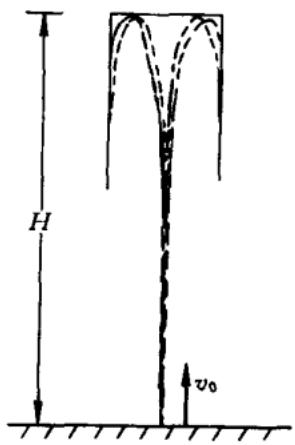
\includegraphics[width=0.15\textwidth]{figures/图2_16.jpg}
\end{center}

\vfill

\textbf{2-20} 质量 $m_{0}$ 、初速 $v_{0}$ 的无动力飞行器在太空尘埃中运动，运动过程中飞行器会吸附尘埃，吸附质量与路程成正比，比例系数为常量 $\alpha$ .

(1) 确定飞行器停止前通过的总路程；

(2) 确定飞行器运动速度与时间的关系.



\vfill

\newpage

\textbf{2-21} 长 $l$ 、质量线密度为 $\lambda$ 的匀质软绳，开始时两端 $A$ 和 $B$ 一起悬挂在固定点上。使 $B$ 端脱离悬挂点自由下落，当如图所示， $B$ 端下落高度 $x < l$ 时，试求悬挂点所受拉力 $T$ 的大小。

\begin{center}
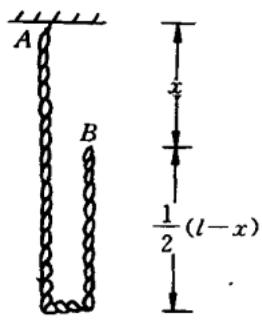
\includegraphics[width=0.15\textwidth]{figures/图2_17.jpg}
\end{center}

\vfill

\textbf{2-22} 盛有水的两个桶 $A$, $B$ 用足够长的轻绳挂在无摩擦定滑轮两侧，$A$, $B$ 质量同为 $m_{0}$ ，已包括桶内水的质量 $m_{0}/2$ ，初始状态系统静止。如图所示，某时刻开始 $A$ 桶内的水从桶底小孔无相对速度地流出，流出质量与时间成正比，比例系数为 $\alpha$ 。试求当 $A$ 桶内的水刚好流完时，$A$ 桶上升速度 $v_{e}$ 。

\begin{center}
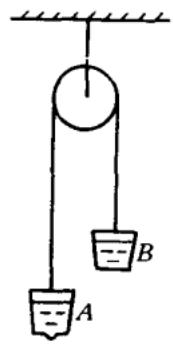
\includegraphics[width=0.15\textwidth]{figures/图_2_18.jpg}
\end{center}

\vfill

\newpage

\section*{B 组}
\vspace{0.3cm}
\textbf{2-23} 系统如图所示, 滑轮与细绳的质量均可略, 绳不可伸长. 设系统所有部位都没有摩擦, 物体 $B$ 借助于固定在大滑块 $C$ 右侧的导轨被限定沿 $C$ 的右侧面运动, 试求大滑块 $C$ 的运动加速度 $a_{c}$ .

\begin{center}
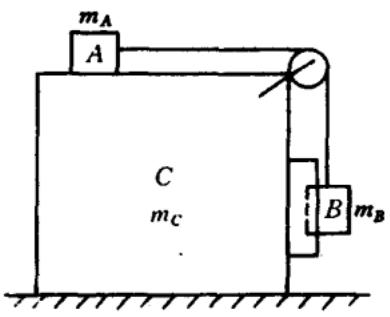
\includegraphics[width=0.2\textwidth]{figures/图2_19.jpg}
\end{center}

\vfill

\textbf{2-24} 如图所示, $xy$ 平面是一绝缘水平面, $z$ 轴竖直向上, 在 $A(x_0,0,0)$ 处放置一电量为 $-q < 0$ , 质量可略的小物块, 物块与水平面间的摩擦因数为 $\mu$ , 物块与一细线相连, 细线的另一端 $B$ 穿过位于坐标原点 $O$ 的光滑小孔, 在水平面下方. 空间加一匀强电场, 场强 $E$ 的方向垂直于 $x$ 轴, 与 $z$ 轴夹角为 $\theta < \pi / 2$ , 且有 $\mu = \tan \theta$ . 今竖直向下缓慢拉动细线 $B$ 端, 使物块在水平面上移动过程的任一位置都可近似认为物块处于力平衡状态. 已知物块的移动轨迹是一条圆锥曲线, 试求其轨迹方程. (物块在电场中受力为 $F = -qE$ .)

\begin{center}
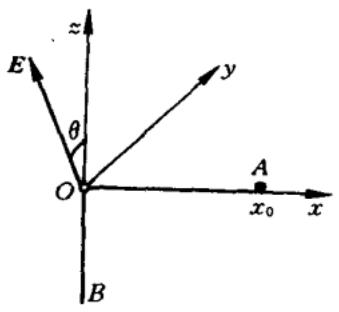
\includegraphics[width=0.2\textwidth]{figures/图2_21.jpg}
\end{center}

\vfill

\newpage

\textbf{2-25} 如图所示, 平而薄的匀质圆板放在水平桌面上, 圆板绕着过中心 $O$ 的竖直轴旋转, $O$ 点沿桌面运动. 如果圆板与桌面间的摩擦因数处处相同, 试证圆板所受合摩擦力的方向必与 $O$ 点运动方向相反.

\begin{center}
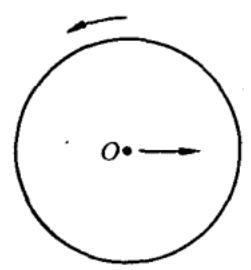
\includegraphics[width=0.2\textwidth]{figures/图2_25.jpg}
\end{center}

\vfill

\textbf{2-26} 质量同为 $m$ 的两个小球, 各自在空气中以速率 $v$ 运动时所受阻力大小为 $f = \alpha mv$ , 其中 $\alpha$ 是一个常量. 使两球位于同一竖直线上, 球 1 在球 2 上方 $h$ 处, 球 2 离地足够高, 在自由释放球 1 的同时, 以初速度 $v_0$ 将球 2 竖直向上抛出. 试问经多长时间 $t_0$ , 两球相遇?


\vfill

\newpage

\textbf{2-27} 在静止的车厢内有一辐角为 $\theta (0 < \theta < 90^{\circ})$ 的圆锥摆，当摆球处于图2-29的最左位置时车厢开始以常量 $a$ 向右作水平匀加速运动.试问摆球相对车厢能否恰好从此时刻开始，以某 $\theta^{\prime}(0 < \theta^{\prime} < 90^{\circ})$ 为辐角作圆锥摆运动？

\begin{center}
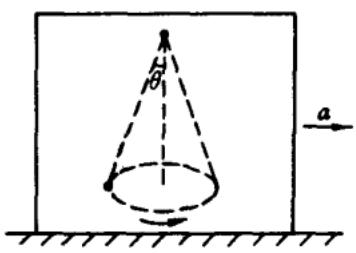
\includegraphics[width=0.2\textwidth]{figures/图2_29.jpg}
\end{center}

\vfill

\textbf{2-28} 盛满同种液体的大容器以恒定的角速度 $\omega$ 绕着一固定轴旋转, 稳定后设液体密度 $\rho_{0}$ 仍可近似认为处处相同.

(1)如图所示，在容器中以转轴与某旋转平面交点为坐标原点，设置径向坐标轴 $x$ ，沿 $x$ 方向取一细长条液柱，它的两端坐标分别为 $x_{1}$ 和 $x_{2}$ ，并且 $x_{2} > x_{1} \gg (x_{2} - x_{1})$ ，截面积同为 $S$ ，试求此液柱所受离心力 $\pmb{F}_{\mathrm{c}}$

(2) 不计重力, 计算 $x$ 处液体压强 $p(x)$ ;

(3) 将图 2-31 中的细液柱置换为外加的固态或液态细柱体, 不计重力, 计算它受到的 $\rho_{0}$ 液体施加的浮力 $F$.

\begin{center}
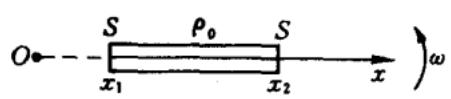
\includegraphics[width=0.3\textwidth]{figures/图2_31.jpg}
\end{center}

\vfill

\newpage

\textbf{2-29} 如图所示, 质量 $m_{1}$ 的航天飞机 $A$ 绕地球作匀速圆周运动, 轨道半径 $R$ , 从航天飞机伸出长 $L \ll R$ 的刚性杆, 杆端固定质量 $m_{2} \ll m_{1}$ 的卫星 $S$ . $A-S$ 系统的位置用 $\alpha$ 角表示, $\alpha$ 是杆与 $A$ 和地心连线之间的夹角. 试求 $A-S$ 系统的平衡位置, 并讨论平衡的稳定性. (稍偏离平衡位置, 静态下若有返回趋势者称为稳定平衡, 有远离趋势者称为不稳定平衡, 能停留者称为随遇平衡.)

\begin{center}
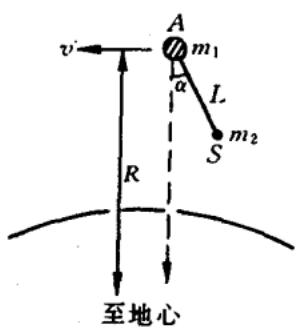
\includegraphics[width=0.2\textwidth]{figures/图2_35.jpg}
\end{center}

\vfill

\textbf{2-30} 不计空气阻力, 近似计算小球从北半球纬度 $\psi$ 上空 $h$ 处自由下落 ( $h \ll R$ (地球半径)), 因受科里奥利力影响产生的落地偏移值.


\vfill

\newpage

\textbf{2-31} 如图所示, 四个质量同为 $m$ 的小球, 用长度相同且不可伸长的轻绳连结成菱形 $ABCD$ , 静放在光滑的水平面上. 今突然给小球 $A$ 一个历时极短沿 $CA$ 方向的冲击, 使 $A$ 获得速度 $v$ . 已知 $\angle BAD = 2\alpha \left( \alpha < \frac{\pi}{4} \right)$ , 试求系统受冲击后瞬间具有的动量 $p$ 以及 $B, C, D$ 球各自速度 $v_B, v_C, v_D$ .

\begin{center}
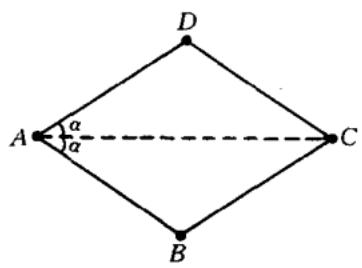
\includegraphics[width=0.2\textwidth]{figures/图2_37.jpg}
\end{center}

\vfill

\textbf{2-32} 从地面发射的炮弹在达到最高点处炸裂成质量相同的两块, 第一块在炸裂后 1 $s$ 落到爆炸点正下方的地面上, 该处与发射点的距离为 $s_{1}=1000$ $m$. 已知最高点距地面高度 h=19.6 $m$, 忽略空气阻力,试求第二块的落地点与发射点的距离.


\vfill

\newpage

\textbf{2-33} 船静止在水面上, 人从船的一端走到另一端, 再返回这一端, 若不计水的阻力, 船往返合成位移为零. 真实情况下水有阻力, 如果来回走的快慢不一样, 船就有可能获得非零的合成位移. 水的阻力较复杂, 可以改取水平地面上有摩擦的长木板, 板上的小物块替换人, 组合成较初等的题目.

如图所示, 质量 M=3m, 长 2l 的均匀长木板静止在水平地面上, 两者间摩擦因数 $\mu=1/8$ . 板的右端有一质量 $m$ 的小物块, 从静止出发通过与木板的某种相互作用机制, 相对木板以朝左的恒定加速度 $a = \frac{1}{2}\alpha g$ 运动，其中 $\alpha > 1$ 是一个不变的参数。小物块到达板中央后，立即改成以 $a = \frac{1}{2}\alpha g$ 的反向加速度继续相对木板运动到左端停下，直到木板在地面上不再运动为止。

(1) 计算木板在地面上朝右的总位移大小 $s_{右}$ ;

(2) 若小物块再以同样方式从板的左端运动到板的右端, 只是将 $a$ 换成 $a' = \frac{1}{2} \alpha' g, \alpha' > 1$ , 导出此过程中木板朝左总位移大小 $s_{\text{左}}$ ;

(3) 小物块如上所述, 在木板上往返一次, 确定木板在地面上合成位移的方向和大小 $s$.

\begin{center}
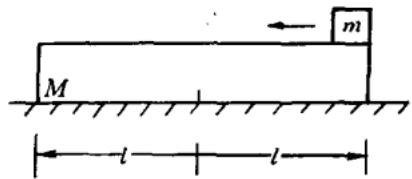
\includegraphics[width=0.3\textwidth]{figures/图2_39.jpg}
\end{center}

\newpage

\textbf{2-34} 球状小水滴在静止的雾气中下落, 下落过程中吸附了全部所遇到的水分子. 设水滴始终保持球状, 雾气密度均匀, 略去空气的黏力, 重力加速度 $g$ 视为不变, 试证经过足够长时间后, 水滴下落加速度趋于稳定值, 并求出此值. 已知满足方程

\[
\frac {\mathrm{d} ^ {2} y}{\mathrm{d} x ^ {2}} + \frac {A}{y} \left(\frac {\mathrm{d} y}{\mathrm{d} x}\right) ^ {2} = B
\]

的函数 $y(x)$ ，其解为

\[
y = (C _ {1} x + C _ {2}) ^ {\frac {1}{A + 1}} + \frac {B}{2 (2 A + 1)} x ^ {2},
\]

其中 $C_1, C_2$ 是两个待定的积分常数.

\vfill

\newpage
